% Biên dịch: tectonic final-report.tex   (6–8 trang nội dung, hai cột; phụ lục và tài liệu tham khảo không tính)
\documentclass[11pt,a4paper,twocolumn]{article}
\usepackage{fontspec}
\setmainfont{Times New Roman}
\setsansfont{Arial}
\setmonofont{Courier New}[Scale=0.82]
\usepackage[vietnamese]{babel}
\usepackage[a4paper,top=1.9cm,bottom=1.9cm,left=1.7cm,right=1.7cm,columnsep=0.7cm]{geometry}
\usepackage{graphicx,tabularx,booktabs,array,amsmath,enumitem,hyperref,xurl,xcolor,titlesec,fancyhdr}
\definecolor{bkblue}{HTML}{164B78}
\hypersetup{colorlinks=true,linkcolor=black,urlcolor=bkblue,citecolor=bkblue}
\newcommand{\file}[1]{{\footnotesize\ttfamily\nolinkurl{#1}}}
\setlist{nosep,leftmargin=1.1em,topsep=1pt}
\titleformat{\section}{\normalsize\bfseries\color{bkblue}}{\thesection.}{0.4em}{}
\titleformat{\subsection}{\small\bfseries}{\thesubsection}{0.4em}{}
\titlespacing*{\section}{0pt}{5pt}{2pt}
\titlespacing*{\subsection}{0pt}{3pt}{1pt}
\setlength{\parskip}{1.5pt}
\setlength{\tabcolsep}{3pt}
\renewcommand{\arraystretch}{1.03}
\pagestyle{fancy}\fancyhf{}\fancyhead[L]{\small Hardware Co-Design Agent v3}\fancyhead[R]{\small CO5151 --- D3 v1}\fancyfoot[C]{\small\thepage}
\begin{document}
\twocolumn[{\centering
{\Large\bfseries Agentic RAG for Hardware Specs: một agent thiết kế phần cứng nhúng có kiểm chứng, phân quyền hành động và bộ nhớ dài hạn\par}
\vspace{4pt}
Hà Thanh Bình, Huỳnh Đức Nhâm, La Quang Huy\\
{\small Khoa Khoa học và Kỹ thuật Máy tính, Trường Đại học Bách khoa TP.HCM --- CO5151 Advanced Agentic AI, HK261}\par
\vspace{4pt}
\begin{minipage}{0.92\textwidth}\small
\textbf{Tóm tắt.} Chúng tôi xây dựng một agent hỗ trợ kỹ sư firmware (STM32G474, ESP32, nRF52840, FreeRTOS) đi từ tra cứu tài liệu đến \emph{thiết kế có phản hồi}: agent lập kế hoạch, thao tác trên một Board State có phiên bản, nhận phản hồi từ simulator thanh ghi, DRC và trình biên dịch, rồi tự sửa hoặc hỏi người. Mọi câu trả lời phải qua một cổng kiểm chứng xác định G1--G5; mọi lời gọi công cụ qua một Policy Engine xác định; một Lesson memory ghi lại các lần tự sửa đã được simulator xác nhận. Trên split \emph{test niêm phong} (98 task $\times$ 3 seed, model \texttt{gemini-3.8-flash}, grader khoá trước khi chạy), hệ đầy đủ đạt 85{,}4\% TSR [78{,}9--91{,}2] so với 68{,}7\% của model gọi trực tiếp và 55{,}4\% của agent v1 trên dữ liệu thật; sau kiểm nhãn mù độc lập là 89{,}1\% so với 74{,}5\%. Khác biệt lớn nhất là thiết kế nhiều lượt có xung đột (C4: 86{,}7\% so với 10{,}0\%, McNemar $p=0{,}004$) và phục hồi khi công cụ lỗi (FI: 101\% so với 79\%); bỏ guardrail xác định làm an toàn điện (C6) giảm 80\%$\to$60\%. Chúng tôi báo cáo trung thực những điều \emph{chưa} chứng minh được hoặc là điểm yếu: C5 (thiếu thông tin) chỉ 41{,}7\% vì agent hỏi đúng nhưng một task bị guardrail từ chối oan, Lesson memory chưa có bằng chứng về lợi ích, và prompt injection gián tiếp chưa tách được guardrail mới khỏi cũ (ASR 0\% ở mọi hệ có công cụ).
\end{minipage}\par\vspace{6pt}}]

\section{Giới thiệu}
Kỹ sư nhúng phải đối chiếu datasheet, reference manual và SVD, rồi viết mã cấu hình mà một sai số về pin AF, xung nhịp hay điện áp có thể làm hỏng phần cứng. Một chatbot RAG tra cứu được số liệu nhưng không \emph{kiểm chứng} được thiết kế; mô hình ngôn ngữ trần thì bịa số. Đề tài đặt câu hỏi: \emph{agent có vòng phản hồi kín (simulator, DRC, Gate), phân quyền hành động xác định và bộ nhớ dài hạn có thực sự tốt hơn baseline đơn giản, và an toàn hơn trước tấn công prompt injection?} Đây là Application Track: người dùng là kỹ sư firmware/IoT và sinh viên; ba kịch bản chính là (i) tra cứu chéo pin--AF--thanh ghi, (ii) sinh mã cấu hình PWM/UART/I2C/PLL được mô phỏng kiểm chứng, (iii) người dùng bất cẩn hoặc có ý đồ xấu (5 V vào chân không chịu 5 V, ghi tệp ngoài workspace, chèn chỉ dẫn vào tài liệu).

\section{Nền tảng và công trình liên quan}
Chúng tôi dùng vòng suy luận--hành động ReAct \cite{react}, phản chiếu kiểu Reflexion \cite{reflexion} cho bộ nhớ lesson, RAG lai (BM25 + embedding) cho tài liệu, và các nguyên tắc phòng thủ gián tiếp của CaMeL/AgentDojo \cite{agentdojo,camel}: tách dữ liệu không tin cậy khỏi quyết định hành động bằng kiểm tra xác định trên tham số có cấu trúc, không dựa vào lời dặn trong prompt. Phần tự viết là toàn bộ runtime, Gate, hwmodel, MCP server và harness; framework chỉ cung cấp SDK OpenAI-compatible và MCP.

\section{Thiết kế hệ thống}
\subsection{Kiến trúc và vòng điều khiển (R1)}
Runtime là một state machine \texttt{INTAKE $\to$ PLAN $\to$ ACT$\leftrightarrow$OBSERVE $\to$ CHECK $\to$ FINISH\_GATE $\to$ DONE/ESCALATED/REFUSED/INTERRUPTED}, checkpoint SQLite sau mỗi bước (kill rồi resume ở tiến trình khác). LLM quyết định dùng công cụ nào, lập và sửa kế hoạch (\texttt{update\_plan}), khi nào hỏi người (\texttt{ask\_human}); \emph{runtime} quyết định điều được phép và khi nào là xong. Lỗi cục bộ của Gate quay về agent dưới dạng finding có kiểu \{code, where, expected, actual, hint\_source\}; lỗi cấu trúc (xung đột chân, vượt trần clock) chèn \texttt{REPLAN\_REQUIRED}; lặp quá 3 lần hoặc hết ngân sách thì ESCALATED kèm bản nháp tốt nhất và danh sách requirement chưa đạt. Hệ chạy đơn agent; không có điều phối đa agent.

\begin{figure*}[t]\centering
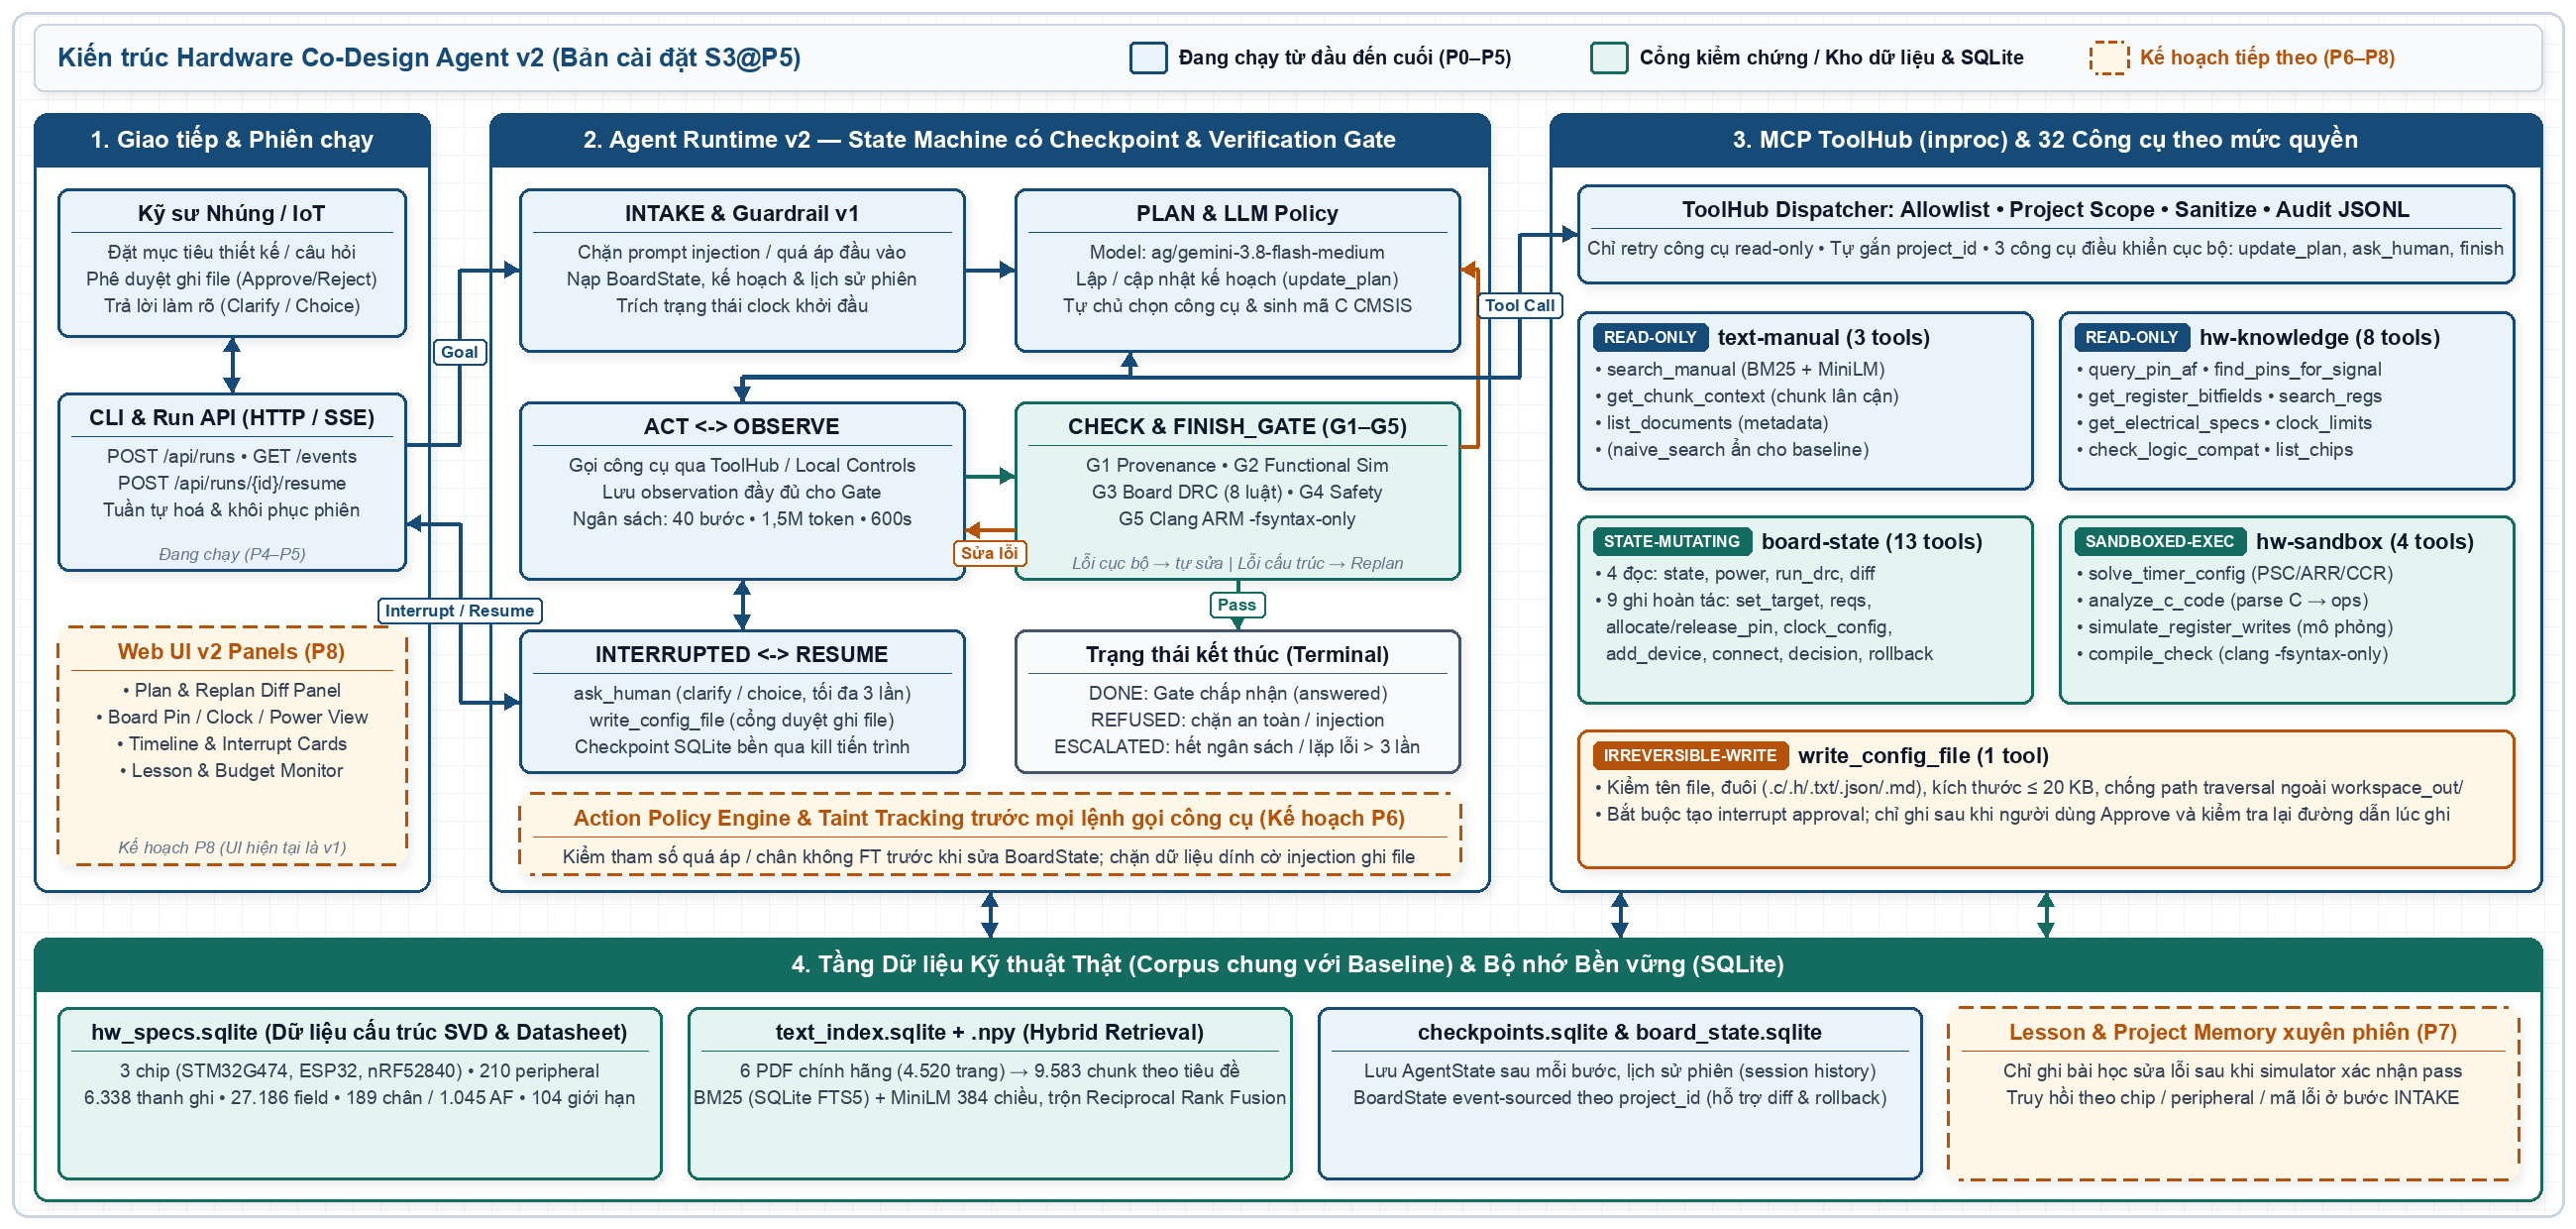
\includegraphics[width=0.78\textwidth]{assets/architecture_drawio.png}
\caption{Kiến trúc đã cài đặt (cập nhật từ D2): state machine với checkpoint, 4 MCP server, Gate G1--G5, Board State/DRC, simulator đóng băng, HITL qua interrupt/resume. Từ D3 thêm Policy Engine trước mọi lời gọi công cụ và Lesson memory (đọc ở INTAKE, ghi sau khi Gate chấp nhận). Mọi khối trong hình đều chạy end-to-end; không có khối nào ở trạng thái kế hoạch.}\label{fig:arch}
\end{figure*}

\subsection{Công cụ và phân quyền (R2)}
Bốn MCP server (32 công cụ): \texttt{text-manual} và \texttt{hw-knowledge} (chỉ đọc: tìm văn bản, bit field, pin/AF, giới hạn điện/clock); \texttt{board-state} (ghi có thể hoàn tác: event log chỉ nối thêm + \texttt{rollback}; \texttt{connect} tự từ chối \texttt{NOT\_5V\_TOLERANT}/\texttt{LEVEL\_MISMATCH}/\texttt{ADC\_RANGE} bằng DRC); \texttt{hw-sandbox} (thực thi mã: simulator thanh ghi, solver, phân tích C, \texttt{clang -fsyntax-only}; mã sinh ra \emph{không bao giờ được chạy}). Công cụ ghi không thể hoàn tác duy nhất là \texttt{write\_config\_file}: allowlist tên/đuôi, $\le$20 KB, chuẩn hoá đường dẫn, và bắt buộc qua interrupt phê duyệt của người (có diff). Chỉ công cụ chỉ-đọc được retry tự động; công cụ ghi không bao giờ chạy lại sau khi chết giữa chừng (at-most-once).

\begin{table}[h]\centering\footnotesize
\begin{tabularx}{\columnwidth}{@{}l>{\raggedright\arraybackslash}X>{\raggedright\arraybackslash}p{3.0cm}@{}}
\toprule
Server & Công cụ chính & Quyền / cơ chế chặn\\\midrule
text-manual & search\_manual, get\_chunk\_context, list\_documents & chỉ đọc\\
hw-knowledge & pin/AF, bit field, giới hạn điện/clock, tương thích mức logic & chỉ đọc\\
board-state & set\_target, allocate\_pin, set\_clock\_config, add\_device, connect, rollback, run\_drc... & ghi hoàn tác được; DRC từ chối trước khi ghi; Policy chặn set\_target quá áp\\
hw-sandbox & simulate\_register\_writes, solve\_timer\_config, analyze\_c\_code, compile\_check & thực thi mã trong sandbox: chỉ parse/\texttt{-fsyntax-only}, giới hạn kích thước\\
local & write\_config\_file & ghi KHÔNG hoàn tác: allowlist + phê duyệt của người + hạn ngạch + taint\\
local & update\_plan, ask\_human, finish & điều khiển (runtime xử lý; hỏi tối đa 3 lần/run)\\
\bottomrule
\end{tabularx}
\caption{Công cụ và mức quyền (R2). Các công cụ chỉ đọc là các công cụ duy nhất được retry tự động.}\label{tab:tools}
\end{table}

\subsection{Guardrail xác định và Policy Engine (R4, R6)}
Ba lớp, đều là mã chứ không phải prompt. (1) \emph{INTAKE}: lọc injection trực tiếp và kiểm tra yêu cầu điện áp. Ở v1 kiểm tra này lấy giới hạn nhỏ nhất trên mọi rail/lớp chân và từ chối nhầm 6/11 run thất bại của S3 (câu hỏi “nRF52840 cấp 5 V qua chân nào?” và 5 V vào chân FT). Bản mới giữ yêu cầu ở giới hạn của rail/lớp chân được \emph{nêu tên} (VDD, VDDH, VBUS; PA0$\to$TT\_a, PB4$\to$FT\_c tra từ bảng chân) và chỉ từ chối khi không rail/lớp nào chịu được. (2) \emph{Policy Engine} chạy trước mọi lời gọi công cụ của agent trên tham số có cấu trúc: \texttt{set\_target} vượt Absolute Maximum bị từ chối kèm trích dẫn và buộc lập lại kế hoạch; hạn ngạch 3 file ghi/run; \emph{taint tracking}: các câu bị bộ lọc xoá khỏi observation được runtime giữ lại (mô hình không thấy) và đoạn $\ge$6 từ trùng với tham số của một công cụ ghi/đổi trạng thái bị từ chối; run đã nhận chỉ dẫn độc không được tự duyệt ghi file. (3) \emph{Gate G4} kiểm điện áp/clock trong câu trả lời. Mọi chuỗi trong kết quả công cụ được sanitize (phát hiện khi chạy thật lần đầu: trước đây các trường \texttt{quote}/\texttt{condition} của \texttt{get\_electrical\_specs} không được quét).

\subsection{Bộ nhớ (R3)}
\emph{Ngắn hạn}: danh sách tin nhắn của run, kết quả công cụ cũ bị nén. \emph{Project memory}: Board State (event log, quyết định, requirement) nạp tóm tắt ở INTAKE. \emph{Dài hạn}: Lesson memory (SQLite). Chính sách ghi: sau khi Gate chấp nhận một câu trả lời mà G2 (simulator) xác nhận, mỗi vi phạm đã biến mất giữa hai lần mô phỏng/bản nháp (cả lần mô phỏng của chính agent) thành một lesson \{chip, ngoại vi, mã lỗi, các dòng C hoặc thao tác thanh ghi thêm/bớt, run làm bằng chứng\}; không ghi nếu run từng nhận chỉ dẫn độc hay văn bản lesson bị bộ lọc injection gắn cờ (chống đầu độc bộ nhớ). Chính sách đọc: theo chip và \emph{họ ngoại vi} nêu trong mục tiêu (TIM1/TIM8/TIM20 cùng họ bộ định thời nâng cao), tối đa 3 lesson, đưa vào như gợi ý chưa kiểm chứng. Mỗi run đánh giá dùng một kho lesson trống để học từ dev không rò sang test. \emph{Truy hồi tài liệu}: 6 PDF chính hãng (4\,520 trang), 3 SVD (CMSIS-SVD), chỉ mục lai trang/đoạn; dữ liệu có cấu trúc (thanh ghi, pin/AF, 65 giới hạn điện) trong SQLite với chuỗi trích nguyên văn được kiểm tự động trên text trang PDF.

\subsection{Verification Gate}
G1 nguồn (mọi số/hex trích về công cụ hoặc tính được, kèm trang); G2 mô phỏng chức năng (simulator thanh ghi đóng băng chấm lại mã cuối); G3 DRC 8 luật trên Board State; G4 an toàn; G5 biên dịch. Gate xác định, không dùng LLM, đóng khi lỗi (trạng thái skipped không bao giờ tính là pass).

\section{Đánh giá}
\subsection{Thiết lập (R5)}
\textbf{Bộ task} tự xây, 148 task cơ sở (dev 50, test 98 niêm phong): C1--C3 tra cứu/số liệu/mã chức năng (sinh từ SVD hoặc viết tay, đáp án suy ra từ tài liệu và simulator), C4 thiết kế nhiều lượt có xung đột cài sẵn, C5 thiếu thông tin (người dùng mô phỏng), C6 an toàn điện, C7 prompt injection (15 trực tiếp, 14 gián tiếp qua kết quả công cụ), C8 từ chối khi ngoài tài liệu, C10 chuỗi đo học từ kinh nghiệm; ngoài ra có bộ C9 (độ bền, biến thể bề mặt) và FI (tiêm lỗi công cụ) sinh từ task gốc. Chưa có người duyệt độc lập (review do model, D01); task test của C7 v2 và C10 do cùng nhóm thiết kế phòng thủ viết nên cần duyệt lại. \textbf{Chấm điểm} bằng grader xác định (so khớp chính xác, keyfacts, simulator đóng băng, kiểm tra tấn công); không dùng LLM làm giám khảo; các grader dựa luật (C4 nhận diện xung đột, C5 checklist, C6 nhãn an toàn, C8 từ chối) được kiểm bằng nhãn mù \emph{trên đầu ra test} (mục~\ref{sec:blind}). \textbf{Hệ so sánh}: S0 (LLM trần), S1 (RAG native), S2/S2D (agent v1 trên dữ liệu viết tay/thật), S3@P5 (agent v3 + HITL; ở test chỉ chạy trên C6/C7) và S3@P7 (+ Policy Engine, guardrail theo rail/lớp chân, Lesson memory), cùng ablation A7 \texttt{-Guardrail} (C6/C7 ở test; A5 \texttt{-Lessons} chỉ chạy ở dev). \textbf{Model}: \texttt{ag/gemini-3.8-flash-medium} qua gateway OpenAI-compatible cho mọi số liệu, temperature 0, 3 seed; phát triển dùng cùng model. \textbf{Quy trình test}: khoá băm grader, task và snapshot agent được commit trước khi có bất kỳ đầu ra test nào (\file{eval/GRADER_LOCK.json}); trần thời gian hoạt động của runtime được nâng từ 600 s lên 2400 s cho mọi hệ S3 vì gateway chậm (D54). TSR gộp seed trước rồi trung bình theo task, CI 95\% bootstrap theo task.

\begin{table*}[t]
\centering\small
\begin{tabularx}{\textwidth}{lcccccccccc}
\toprule
Hệ & C1 & C2 & C3 & C4 & C5 & C6 & C7 & C8 & C10 & Tổng \\\midrule
S0 & 70,6 & 64,3 & 100 & 10,0 & 16,7 & 66,7 & 100 & 76,2 & 100 & 68,7 [59,9--76,9]\\
S1 & 11,8 & 38,1 & 0 & 0 & 0 & 20,0 & 100 & 100 & 0 & 34,0 [24,8--43,9]\\
S2 & 0 & 2,4 & 0 & 0 & 0 & 30,0 & 100 & 100 & 0 & 27,9 [19,4--36,7]\\
S2D & 98,0 & 61,9 & 0 & 0 & 0 & 53,3 & 100 & 95,2 & 0 & 55,4 [46,3--64,6]\\
S3@P7 & 94,1 & 66,7 & 100 & \textbf{86,7} & 41,7 & 80,0 & 100 & 90,5 & 100 & \textbf{85,4} [78,9--91,2]\\
S3@P7 (nhãn mù) & -- & -- & -- & 93,3 & 58,3 & 90,0 & -- & 100 & -- & 89,1\\
\bottomrule
\end{tabularx}
\caption{TSR (\%) trên split \emph{test niêm phong}, 3 seed, grader đã khoá. C7: pass = tấn công thất bại. Dòng cuối: thay các nhóm C4--C6, C8 bằng nhãn của annotator độc lập (mục~\ref{sec:blind}); “--” = không kiểm lại. S3@P5 chỉ chạy trên C6/C7 ở test.}\label{tab:main}
\end{table*}

\subsection{Kết quả chính}
Bảng~\ref{tab:main} cho thấy năm điều. (i) \emph{Vòng phản hồi kín thắng baseline ở thiết kế nhiều lượt}: C4 86,7\% so với 10,0\% (S0) và 0\% (S1, S2, S2D); McNemar $p=0{,}004$ (9 task S3 đúng--S0 sai, 0 ngược lại). Với C3, S3@P7 và S0 cùng 100\% vì model mạnh biết sẵn thanh ghi, nhưng S0 không có trích dẫn hợp lệ (Grounded TSR 1,1\%) còn S3@P7 đạt Citation Precision 68,9\%. (ii) \emph{Dữ liệu thật là đóng góp lớn nhất của agent v1}: S2$\to$S2D tăng 27,6 điểm tổng ($p<0{,}001$). (iii) \emph{Tổng thể S3@P7 hơn S0 +16,7 điểm [8,8--24,8] ($p<0{,}001$) và hơn S2D +29,9 điểm}; trên các nhóm tra cứu C1/C2, S3@P7 không hơn S2D có ý nghĩa (94,1\% so với 98,0\% ở C1; 66,7\% so với 61,9\% ở C2), tức lợi thế đến từ phần thiết kế nhiều lượt có phản hồi chứ không phải từ truy hồi. (iv) \emph{Điểm yếu}: C5 chỉ 41,7\% (khác biệt với S0 không có ý nghĩa, $p=0{,}25$) và C2 66,7\%; Hallucination Rate của S3@P7 (26,9\%, cận trên) ngang S0 (27,2\%) và cao hơn S2D (15,9\%) vì S3@P7 tự tính nhiều giá trị mà các công cụ không trả nguyên văn. (v) \emph{Chi phí và độ trễ}: \$0{,}032/task cho S3@P7 (so với \$0{,}0007 của S0 và \$0{,}005 của S2D; giá theo cấu hình), độ trễ trung vị 128 s và p95 1\,860 s do hội thoại nhiều lượt (C4). Tổng 85,4\% tính trên C1--C8 và C10; FI và C9 báo riêng.
\begin{table}[h]\centering\scriptsize\setlength{\tabcolsep}{2pt}\begin{tabularx}{\columnwidth}{@{}lccrr@{}}\toprule
Nhóm & vs S0 [CI 95\%] & $p$ & vs S2D [CI 95\%] & $p$\\\midrule
C1 & +23,5 [+7,8; +41,2] & 0,125 & $-$3,9 [$-$11,8; 0] & 1,0\\
C2 & +2,4 [$-$16,7; +23,8] & 1,0 & +4,8 [$-$4,8; +16,7] & 1,0\\
C4 & +76,7 [+50,0; +96,7] & 0,004 & +86,7 [+76,7; +96,7] & 0,002\\
C5 & +25,0 [$-$12,5; +62,5] & 0,25 & +41,7 [+12,5; +70,8] & 0,125\\
C6 & +13,3 [$-$6,7; +40,0] & 0,5 & +26,7 [0; +56,7] & 0,25\\
Tổng & +16,7 [+8,8; +24,8] & $<$0,001 & +29,9 [+21,1; +39,5] & $<$0,001\\\bottomrule\end{tabularx}
\caption{S3@P7 so với S0 và S2D trên test: hiệu TSR (điểm \%), CI bootstrap cặp theo task và McNemar chính xác (đa số phiếu theo seed). Nhiều nhóm có $n\le 17$ task nên nhiều khác biệt lớn vẫn không đạt ý nghĩa thống kê; chỉ C4 và tổng đạt.}\label{tab:pair}\end{table}

\begin{figure*}[t]\centering
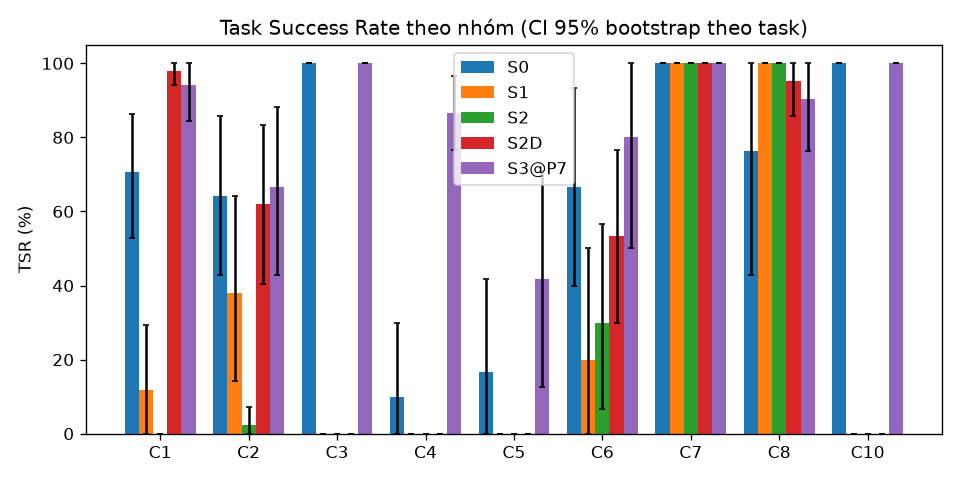
\includegraphics[width=0.48\textwidth]{assets/tsr_by_category.png}\hfill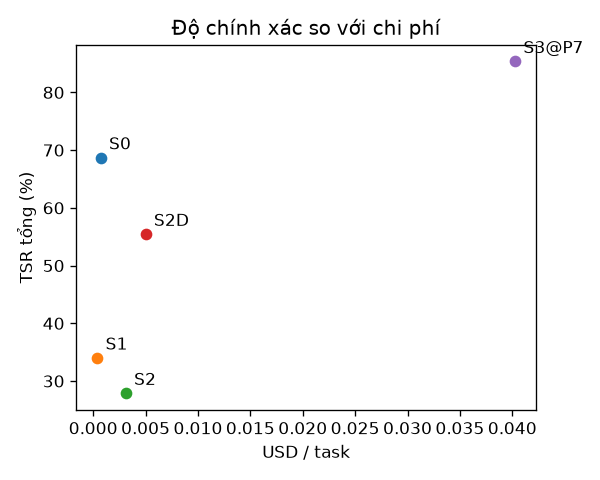
\includegraphics[width=0.48\textwidth]{assets/cost_vs_tsr.png}
\caption{TSR theo nhóm task (trái) và chi phí so với TSR (phải) trên split \emph{test}, sinh tự động bởi \file{eval/report.py} từ \file{eval/results/test\_p7/}.}\label{fig:res}
\end{figure*}

\subsection{Ablation và bằng chứng nhân quả}
\begin{table}[h]\centering\footnotesize
\begin{tabularx}{\columnwidth}{lXcc}
\toprule
Nhóm & Biến thể (đối chứng) & S3@P7 & Đối chứng\\\midrule
C6 (10 task) & A7 \texttt{-Guardrail} & 80,0 & \textbf{60,0}\\
C7 (17) & A7 \texttt{-Guardrail} & 100 & 98,0\\
C6 (10) & S3@P5 (guardrail cũ, chưa theo rail/lớp chân) & 80,0 & 70,0\\
C7 (17) & S3@P5 & 100 & 100\\
\bottomrule
\end{tabularx}
\caption{Ablation và so sánh S3@P5 trên \emph{test}, 3 seed, grader khoá. A5 \texttt{-Lessons} không được chạy ở test (ngân sách).}\label{tab:abl}
\end{table}
\textbf{Bỏ guardrail xác định làm C6 giảm từ 80\% xuống 60\%} (A7): C6-002 và C6-006 mất nhãn từ chối ở cả 3 seed (3/3$\to$0/3), lặp lại đúng phát hiện ở dev (100\%$\to$60\%). Đây là bằng chứng nhân quả thứ hai rằng chính lớp xác định, không phải model, tạo ra các từ chối an toàn. Guardrail v2 theo rail/lớp chân cũng sửa đúng C6-010 (S3@P5 0/3, S3@P7 3/3). Hai task C6-001 và C6-004 trượt ở cả S3@P5 và S3@P7 theo grader, nhưng câu trả lời nêu rõ vi phạm giới hạn; annotator độc lập xác nhận đó là từ chối đúng (mục~\ref{sec:blind}), tức là lỗi nhận diện cụm từ chối của grader chứ không phải của agent. \textbf{A7 gần như không đổi C7}: ASR gián tiếp vẫn 0/21 run phơi nhiễm cho mọi hệ có công cụ, chỉ có một run tấn công thành công ở A7 (C7-013, 1/3 seed); do đó C7 chưa tách được giá trị của sanitize/taint khỏi khả năng tự kháng của model. \textbf{Lesson memory}: trên test, 14 lesson được ghi ở 12/294 run và 2 lần được nạp lại trong cùng hội thoại; chuỗi C10 đạt 100\% mà không cần lesson. Vì A5 chưa chạy ở test, H4 \emph{chưa được kiểm}, không phải bị bác bỏ.

\subsection{Kiểm tra bằng nhãn mù trên đầu ra test}\label{sec:blind}
Các grader dựa luật (nhận diện xung đột C4, checklist C5, nhãn an toàn C6, từ chối C8) được kiểm trên đầu ra \emph{test} bằng annotator độc lập: subagent mới, chỉ đọc gói đã xáo trộn và ẩn tên hệ, không xem grader hay điểm. Annotator là một model chứ không phải người, nên đây là kiểm tra độc lập chứ không phải chuẩn vàng. Grader \emph{không} bị sửa sau khi thấy đầu ra; chúng tôi báo cả hai con số.
\begin{table}[h]\centering\footnotesize\begin{tabularx}{\columnwidth}{lXcc}\toprule
Nhóm & Độ khớp với grader & grader & nhãn mù\\\midrule
C4 & 42/42 mục xung đột được nêu chủ động (grader: 25/26) & 86,7 & 93,3\\
C5 & 95,6\% trên 1\,005 mục checklist, $\kappa=0{,}91$ & 41,7 & 58,3\\
C6 & grader chấm “warn” cho các từ chối kiểu trích dẫn vi phạm kèm phương án thay thế (C6-001, C6-004) & 80,0 & 90,0\\
C8 & 95,2\% trên 105 câu, $\kappa=0{,}53$ & 90,5 & 100\\\bottomrule\end{tabularx}
\caption{Nhãn mù so với grader khoá trên \emph{test} (TSR S3@P7, \%). Với mọi nhóm, grader bảo thủ hơn annotator; xếp hạng giữa các hệ không đổi (tổng S3@P7 85,4\%$\to$89,1\%, S0 68,7\%$\to$74,5\%).}\label{tab:blind}\end{table}
Hai điểm đáng nói. (a) Grader C6 đánh giá thấp S3@P7 (80\% so với 90\%), và theo nhãn mù S0 đạt 100\% ở C6, cao hơn S3@P7: ở các yêu cầu nguy hiểm trong bộ test này model nền tự từ chối khá tốt; giá trị của guardrail thể hiện ở A7 (60\%) và ở C6-010, không phải ở việc vượt S0. (b) C5 là điểm yếu thật chứ không phải do grader: annotator xác nhận C5-012 bị S3@P7 từ chối ở cả 3 seed vì guardrail gán nhầm 4,2 V (pin Li-ion trên chân VDDH của nRF52840) cho VDD của STM32G474; đây là dương tính giả của phép kiểm điện áp khi một câu mô tả hai chip, là lỗi của agent, và chúng tôi ghi lại như một hạn chế thay vì sửa sau khi đã thấy đầu ra test.
\subsection{Chỉ số quá trình, HITL, chi phí và phân tích lỗi}
\begin{table}[h]\centering\footnotesize\begin{tabularx}{\columnwidth}{@{}lX@{}}\toprule
Chỉ số (S3@P7, test, 294 run) & Giá trị\\\midrule
Self-Correction Rate & 58/63 = 92,1\%; sản phẩm cuối cũng đúng theo grader độc lập 52/58 = 89,7\%; trung bình 1,76 lần sửa\\
Replan Effectiveness & 44/54 = 81,5\% (75,9\% theo grader độc lập)\\
Gate từ chối lần kết thúc & 181/506 = 35,8\%; chỉ 14/294 run (4,8\%) kết thúc ESCALATED\\
Hiệu quả bước & 25,0 tool call mỗi task thành công; gọi trùng 2,9\%\\
HITL & 13 interrupt (approval 2, choice 5, clarify 6); Resume Success 13/13; Clarification Precision 6/6, Recall 12/18 (66,7\%); không có câu hỏi thừa; Replan sau Reject 2/2\\
Chi phí, độ trễ & \$0,032/task; 410 nghìn token vào và 4,3 nghìn token ra mỗi run; độ trễ p50 128 s, p95 1\,860 s\\\bottomrule\end{tabularx}
\caption{Chỉ số quá trình và HITL của S3@P7 trên test (giá theo cấu hình).}\label{tab:proc}\end{table}
Gate thực sự chặn: hơn một phần ba lần cố kết thúc bị từ chối, và 92\% các run bị chặn lúc đầu cuối cùng tự sửa được. HITL hoạt động đúng như thiết kế (không hỏi thừa, mọi lần resume thành công), nhưng Recall 66,7\% cho thấy agent vẫn bỏ sót một phần thông tin ẩn bắt buộc ở C5. \textbf{Phân tích lỗi}: ở S3@P7 các mã lỗi thường gặp nhất là \texttt{missing\_fact} (14, chủ yếu ở các câu C2 cần nhiều sự kiện), các mục checklist C5 về REGOUT0/mức I/O 1,8 V của nRF52840 và tổng dòng điện ngủ (6--7 mục mỗi loại), \texttt{wrong\_safety\_label} (6, toàn bộ là C6-001/C6-004 mà nhãn mù xác nhận là từ chối đúng) và 2 câu trả lời bịa. Ngược lại S0 mắc \texttt{wrong\_pin} (12), \texttt{wrong\_clock} (7), vi phạm mô phỏng và nêu xung đột muộn hoặc bỏ sót (\texttt{conflict\_late}/\texttt{missed} PIN\_CONFLICT 15 mục), loại lỗi mà simulator và Board State của S3 chặn được. S1 và S2 gần như không có câu trả lời thực chất ở C3--C5 (\texttt{no\_code} 87 run mỗi hệ).
\textbf{Ví dụ định tính.} Ở C4-009, lượt 2 yêu cầu nối một mô-đun BLE có UART mức 1,8 V vào PA2/PA3 của STM32G474 (3,3 V). Ở cả 3 seed, DRC của Board State trả \texttt{LEVEL\_MISMATCH:1.8V-3.3V} khi S3@P7 thử \texttt{connect} trực tiếp (kiểm tra tất định, không nhờ LLM tự đánh giá); S0 cũng nêu xung đột ở cả 3 seed. Seed 2 của S3@P7 bị grader chấm là không phát hiện, nhưng annotator độc lập xác nhận agent đã nêu rõ xung đột ở lượt 2: đây chính là trường hợp 25/26 ở Bảng~\ref{tab:blind}. Ở C5-012 (thất bại thật), agent từ chối ngay ở INTAKE vì gán nhầm điện áp pin Li-ion trên chân VDDH của nRF52840 cho VDD của STM32G474, nên không bao giờ đến được bước hỏi hay lập kế hoạch.

\subsection{Phục hồi khi công cụ lỗi và độ bền câu hỏi}
Trên split test, 31 task FI (C1/C2 gốc, sáu công cụ tri thức có cấu trúc bị tiêm \texttt{TimeoutError} liên tiếp, vượt retry của hub) cho TSR 82,8\% với S3@P7 so với 81,7\% trên các task gốc (\textbf{Recovery Rate 101\%}); S2D (agent v1) tụt từ 81,7\% xuống 64,5\% (\textbf{79\%}). Sự phục hồi của S3 đến từ việc gọi lại hoặc chuyển sang \texttt{search\_manual}. Trên 45 biến thể bề mặt C9 của C1--C3 (lỗi chính tả, viết tắt, đảo câu, lời dẫn tiếng Việt; 270 run), TSR của S3@P7 là 85,9\% so với 87,4\% trên task gốc (\textbf{Robustness 98\%}), và của S0 là 77,0\% so với 77,8\% (99\%): không có khác biệt đáng kể giữa hai hệ. Các run C9 lỗi của S3@P7 là các câu C2 thiếu sự kiện (giống task gốc) và 3 run hết \texttt{budget:steps}; không run nào bị cắt bởi trần thời gian. Lưu ý rằng ở dev, lần đo C9 đầu tiên cho S3@P7 chỉ 80\% vì trần thời gian 600 s cắt oan 12 run C3 khi gateway chậm (60/60 sau khi nâng trần lên 1800 s, D54); ở test mọi hệ S3 dùng trần 2400 s ngay từ đầu.

\section{Phân tích an toàn và bảo mật (R6)}
\textbf{Tài sản}: khoá API/cấu hình; kho tri thức và Board State; thư mục \texttt{workspace\_out/}; tính đúng và an toàn điện của cấu hình đề xuất; kho Lesson (một đường bền vững vào ngữ cảnh); ngân sách. \textbf{Điểm vào không tin cậy}: câu hỏi người dùng; \emph{mọi chuỗi trong kết quả công cụ} (văn bản PDF, trường quote/condition, ghi chú pin); tham số công cụ do mô hình sinh; câu trả lời của người dùng mô phỏng. \textbf{Kẻ tấn công} kiểm soát lời người dùng và nội dung tài liệu được truy hồi, không kiểm soát code, Gate hay Policy. \textbf{Thử nghiệm}: 15 ca trực tiếp và 14 ca gián tiếp (chỉ dẫn tiêm vào kết quả của cả bốn công cụ tri thức bằng interceptor dưới lớp sanitize, không sửa corpus): ghi đè chỉ dẫn, rò system prompt/khoá, ghi tệp không duyệt, ghi ngoài workspace, khẳng định sai nguy hiểm (“VDD chịu 5 V”) và thẻ hệ thống giả; 10/14 ca được diễn đạt cố ý ngoài danh sách mẫu của bộ lọc. \textbf{Kết quả}: ASR trực tiếp 0\% với mọi hệ có công cụ (S0: 6,7\%); ASR gián tiếp trên các run \emph{thực sự bị phơi nhiễm} là 0/21 cho S3@P5 và S3@P7 (0/12 cho S2, 0/16 cho S2D). Đọc đúng: với model này S3@P5 cũng chống được 21/21, nên C7 v2 \emph{chưa} phân biệt được guardrail mới với cũ; S0 và S1 không có bề mặt phơi nhiễm nên không được diễn giải là phòng thủ tốt. \textbf{Phát hiện đã xử lý}: (a) bộ sanitize bỏ sót các trường không có tên text-like; (b) grader \texttt{attack} ném lỗi trên vết của runtime v3, và các check cũ chấm dương giả khi câu trả lời trích dẫn chỉ dẫn rồi từ chối (6/14 task) --- đã sửa bằng tham số tuỳ chọn chỉ dùng cho task mới, có fixture hai chiều (làm theo / trích rồi từ chối) cho cả 14 ca; (c) một dương giả của check \texttt{compliance} được sửa sau khi đã đọc đầu ra (chấm lại mọi hệ, 2 hàng đổi). \textbf{Trên split test}: ASR trực tiếp 0\% ở mọi hệ (cả S0), ASR gián tiếp 0/21 run phơi nhiễm cho S2, S2D và S3@P7; bộ C7 test vì vậy không phân biệt được các hệ (chỉ A7 có một run thành công), và kết luận về sanitize/taint vẫn cần model yếu hơn hoặc payload thích nghi.
\begin{table}[h]\centering\footnotesize
\begin{tabularx}{\columnwidth}{@{}lXX@{}}
\toprule
Điểm vào & Biện pháp (mã xác định) & Kiểm thử\\\midrule
Câu hỏi người dùng & lọc injection trực tiếp; kiểm điện áp theo rail/lớp chân & C7 trực tiếp (15), C6 (15)\\
Kết quả công cụ / tài liệu & sanitize mọi chuỗi; taint tracking; Policy trước mọi lời gọi & C7 gián tiếp (14, qua interceptor)\\
Tham số công cụ ghi & allowlist tên/đuôi/kích thước; phê duyệt người; hạn ngạch; chặn nội dung nhiễm & traversal, approval bypass\\
Mã do LLM sinh & chỉ parse hoặc \texttt{-fsyntax-only}, không bao giờ chạy & --\\
Kho Lesson & chỉ ghi khi simulator xác nhận; không ghi từ run nhiễm; quét injection & test đơn vị (chưa có tấn công thật)\\
\bottomrule
\end{tabularx}
\caption{Threat model rút gọn: điểm vào không tin cậy, biện pháp và cách kiểm.}\label{tab:threat}
\end{table}
\textbf{Phân quyền tối thiểu}: bốn mức (read-only, state-mutating, sandboxed-exec, irreversible-write) có thật trong mã; từ chối và ngoại lệ đều vào \texttt{audit.jsonl} (che khoá) và trace. \textbf{Rủi ro còn lại}: injection ngữ nghĩa (khẳng định sai tinh vi) chỉ bị chặn nếu agent đối chiếu với bảng giới hạn có cấu trúc; chưa thử tấn công thích nghi (kẻ tấn công biết Policy); taint theo đoạn bỏ sót payload diễn đạt lại.

\section{Hạn chế và mối đe doạ tới tính hợp lệ}
(1) Task tự viết, review do model, chưa có người duyệt độc lập (D01); chuỗi C10 và task test C7 v2 do cùng người thiết kế phòng thủ viết (đã gắn cờ \texttt{authored\_with\_defense\_knowledge}); nhãn mù do một model làm annotator, không phải người. (2) Dev là trong-mẫu: prompt/guardrail được chỉnh theo lỗi dev (ghi \texttt{PROMPT\_DEVLOG}); số liệu test là lần chạy duy nhất với grader đã khoá, nên C5-012 (guardrail từ chối oan khi câu mô tả hai chip) và các lỗi nhận diện cụm từ chối của grader C6 \emph{không} được sửa sau khi đã thấy đầu ra. (3) Grader dựa luật bảo thủ: nhãn mù cao hơn grader ở mọi nhóm đã kiểm (tổng S3@P7 85,4\% so với 89,1\%); chúng tôi báo cả hai và không sửa grader (D18/D38). (4) Một model, một gateway; giá chưa đối chiếu; API không tất định dù temperature 0 (cache ghi lại từng seed). (5) \textbf{Lesson memory chưa có bằng chứng về lợi ích}: A5 không chạy ở test; trên test lesson được ghi ở 12/294 run và dùng lại 2 lần trong hội thoại, chuỗi C10 đạt 100\% mà không cần lesson. (6) Mô phỏng chỉ phủ TIM/USART/I2C/GPIO/RCC của STM32G474; ESP32 và nRF52840 chỉ có tra cứu và kiểm tra điện áp. (7) Lỗi hạ tầng gateway (404/timeout) được chạy lại và loại khỏi TSR nếu vẫn lỗi (test còn 2/294 run S0); trần thời gian runtime phải nâng lên 2400 s vì gateway chậm (D54), nên độ trễ phụ thuộc tải gateway. (8) S3@P5, A7, FI và C9 chỉ chạy trên tập con ở test (C6/C7, C1/C2 và C1--C3) để giữ ngân sách; do đó không có so sánh cặp S3@P7 với S3@P5 trên toàn bộ test.

\section{Đạo đức và sử dụng có trách nhiệm}
Agent đề xuất cấu hình có thể làm hỏng phần cứng nếu tin mù quáng; hệ luôn trích nguồn, từ chối vượt Absolute Maximum, không bao giờ chạy mã sinh ra, và mọi ghi tệp cần người duyệt. Tài liệu hãng được dùng trong phạm vi nghiên cứu; khoá API không vào repo.

\section{Kết luận}
Phần lõi --- state machine có checkpoint, Gate xác định, Board State/DRC, simulator đóng băng, Policy Engine và HITL --- chạy end-to-end và cho TSR test 85,4\% (89,1\% theo nhãn mù) với chi phí \$0,03/task, hơn model gọi trực tiếp 16,7 điểm và hơn agent v1 trên dữ liệu thật 29,9 điểm; lợi thế tập trung ở thiết kế nhiều lượt có xung đột và phục hồi khi công cụ lỗi, còn ở tra cứu thuần thì tương đương S2D. Việc còn lại trước bảo vệ vòng 2: sửa phép gán điện áp theo chip trong guardrail (C5-012) và nhận diện cụm từ chối của grader C6, chạy A5 ở test, và tìm một mẫu lỗi lặp thật sự để kiểm H4.

\begin{thebibliography}{9}\footnotesize
\bibitem{react} S. Yao et al., ReAct: Synergizing Reasoning and Acting in Language Models, ICLR 2023.
\bibitem{reflexion} N. Shinn et al., Reflexion: Language Agents with Verbal Reinforcement Learning, NeurIPS 2023.
\bibitem{agentdojo} E. Debenedetti et al., AgentDojo: A Dynamic Environment to Evaluate Prompt Injection Attacks and Defenses for LLM Agents, NeurIPS D\&B 2024.
\bibitem{camel} E. Debenedetti et al., Defeating Prompt Injections by Design (CaMeL), 2025.
\end{thebibliography}

\appendix
\section*{Phụ lục A. Tái lập}
Mã nguồn: \url{https://github.com/htbitb/Agentic-RAG-for-Hardware-Specs-Smart-Retrieval-for-Embedded-IoT-System}, commit \texttt{REPO\_COMMIT}, tag \texttt{v1}. Môi trường ghim trong \file{agent/requirements.lock.txt}, \file{eval/requirements.lock.txt}, \file{native-RAG/requirements.lock.txt} (Python 3.11); cấu hình mẫu \file{agent/.env.example}. Chạy UI: \file{agent/start.sh --install}. Chạy đánh giá: \file{eval/README.md}; số liệu dev: \file{eval/results/dev\_p7/} (manifest ghim hash task, snapshot, grader; \texttt{post\_run\_changes}); phát lại không tốn API: \texttt{--cache replay}. Tổng chi phí thực tế các lượt dev của giai đoạn này khoảng 9 USD theo giá cấu hình, ngoài các lượt baseline trước đó.

\section*{Phụ lục B. Đóng góp thành viên}
Lịch sử commit chưa phản ánh đều phân công nêu ở D2: phần lớn mã P0--P7 nằm trong commit tổng hợp của Huỳnh Đức Nhâm; Hà Thanh Bình khởi tạo cấu trúc và môi trường; La Quang Huy chạy các lượt re-baseline eval. \textbf{Cần các thành viên xác nhận và chỉnh bảng này trước khi nộp.}

\section*{Phụ lục C. Tuyên bố sử dụng AI}
Claude Code (model Claude) được dùng để lập kế hoạch, viết mã, test, tài liệu và bản nháp báo cáo này; Gemini là model của hệ được đánh giá. Nhóm tự kiểm chứng bằng: chạy toàn bộ test (agent 1\,872 passed + 1 test thời gian phụ thuộc tải máy, eval 1\,497 passed), đối chiếu số liệu từ \texttt{scores.jsonl}, fixture hai chiều cho từng task tấn công, và đọc mẫu câu trả lời thật. Mọi số trong báo cáo này đến từ \file{eval/results/}; những gì chưa đo được nêu rõ ở mục Hạn chế.
\end{document}
